\chapter{细胞初探}\label{ch:g5:first-look-at-cells}

看看你的手背：\omterm{def:g1:the-five-senses:sense}{皮肤}光滑，表面完整无缝。
现在想象一个能放大一千倍的放大镜。
这片无缝的表面会溶解成
一片由许多微小隔间组成的“路面”，隔间像石板一样紧密拼合；
——你在本书中见过的每一种\omterm{def:g1:living-or-not:living}{生物}，从\omterm{prop:g4:plants-without-seeds:damp}{苔藓}到鲸，
都是这样铺成的。生物学最大的秘密
就藏在微小之中。

\section{生物都由细胞构成}

\begin{definition}[细胞]\label{def:g5:first-look-at-cells:cell}
\emph{细胞}\index{细胞}是\omterm{def:g1:living-or-not:living}{生物}体中最小的活的构件，
几乎所有细胞都小到肉眼无法看见。
\omterm{def:g1:living-or-not:living}{生物}体由细胞构成，就像墙由砖块砌成一样。
你自己的身体由几十万
亿个细胞组成。
\end{definition}

\begin{proposition}[细胞学说]\label{prop:g5:first-look-at-cells:principle}
每一种\omterm{def:g1:living-or-not:living}{生物}都由\omterm{def:g5:first-look-at-cells:cell}{细胞}构成：每一种\omterm{def:g1:animals-around-us:animal}{动物}、
每一种\omterm{def:g1:plants-around-us:plant}{植物}、每一种蘑菇，直至只由
\emph{一个}\omterm{def:g5:first-look-at-cells:cell}{细胞}组成的\omterm{def:g1:living-or-not:living}{生物}。这种共同的构成方式
是\emph{生命的统一性}\index{生命的统一性}的重要标志：
雏菊与鲸鱼看上去多么不同，在微观层面，
它们都由同一类微小的活的单位构成。
\end{proposition}
\admitted

\begin{example}[细胞有多小？]\label{ex:g5:first-look-at-cells:small}
你身体中一个典型的\omterm{def:g5:first-look-at-cells:cell}{细胞}大约只有
五十分之一毫米。把 $50$ 个这样的\omterm{def:g5:first-look-at-cells:cell}{细胞}排成一列，恰好长一毫米
——连一个铅笔点都能盖住整列\omterm{def:g5:first-look-at-cells:cell}{细胞}。这就是为什么在人类历史的大部分时间里，
没有人怀疑过\omterm{def:g5:first-look-at-cells:cell}{细胞}的存在：
生命的构件比眼睛能看到的最小斑点还要小。
\end{example}

\section{揭示细胞的仪器}

\begin{definition}[显微镜]\label{def:g5:first-look-at-cells:microscope}
\emph{显微镜}\index{显微镜}是一种仪器，
其透镜能将极小的物体放大数百倍。将它对准\omterm{def:g1:living-or-not:living}{生物}材料的薄片时，
人们第一次看到了从前任何眼睛都未曾见过的东西：
\omterm{def:g5:first-look-at-cells:cell}{细胞}。这个名称本身是由一位早期观察者提出的，
他觉得软木薄片中的小隔间很像修道士的小房间——
于是称之为\emph{\omterm{def:g5:first-look-at-cells:cell}{细胞}}。
\end{definition}

\begin{omfigure}
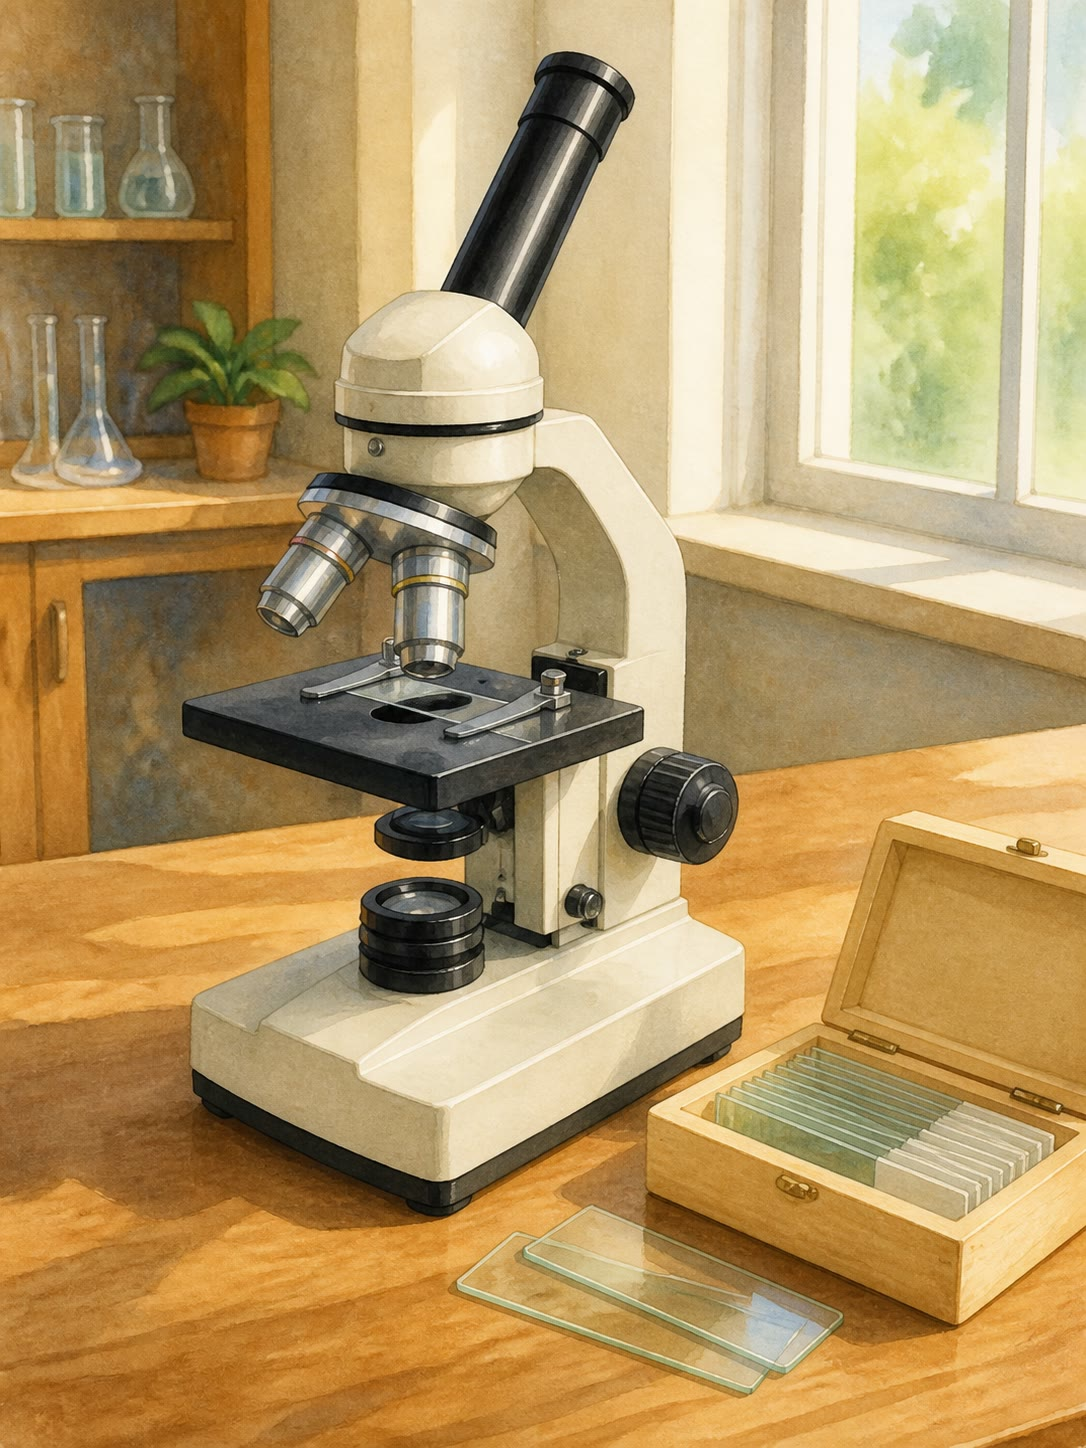
\includegraphics[width=0.44\linewidth]{images/book1/ai/g5-cells-microscope.jpg}

{\small 揭示\omterm{def:g5:first-look-at-cells:cell}{细胞}的仪器：透镜、光线，
以及放在载玻片上的薄片。}
\end{omfigure}

\begin{example}[显微镜下的两个经典观察]\label{ex:g5:first-look-at-cells:classics}
任何一台学校的\omterm{def:g5:first-look-at-cells:microscope}{显微镜}都能重复的两项观察：撕下一小片
洋葱内表皮，可以看到整齐排列的砖块状\omterm{def:g5:first-look-at-cells:cell}{细胞}，
一面墙挨着一面墙；轻轻刮取口腔内侧的黏膜，
看到散开的、较圆的\omterm{def:g5:first-look-at-cells:cell}{细胞}——那是你自己的\omterm{def:g5:first-look-at-cells:cell}{细胞}。
\omterm{def:g1:plants-around-us:plant}{植物}与\omterm{def:g1:animals-around-us:animal}{动物}并排观察，两者都由\omterm{def:g5:first-look-at-cells:cell}{细胞}构成。
\end{example}

\begin{omfigure}
\begin{minipage}[t]{0.48\linewidth}\centering
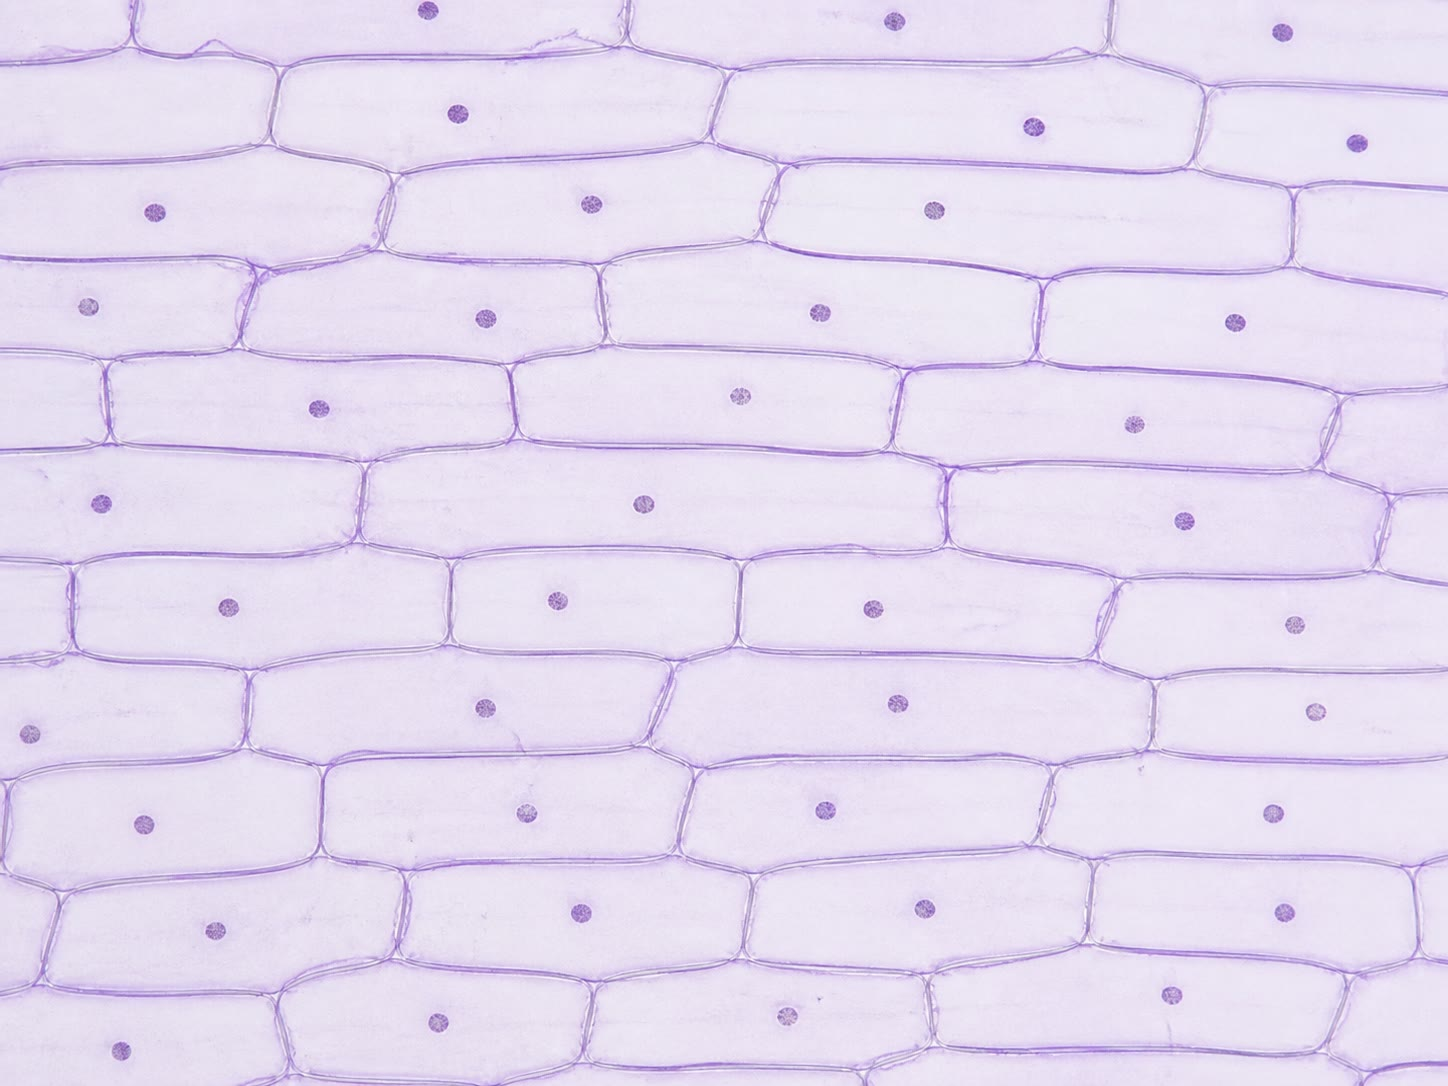
\includegraphics[width=\linewidth]{images/book1/ai/fig-onion-cells.jpg}

{\small 洋葱表皮：砖块状\omterm{def:g5:first-look-at-cells:cell}{细胞} \\ 整齐排列}
\end{minipage}\hfill
\begin{minipage}[t]{0.48\linewidth}\centering
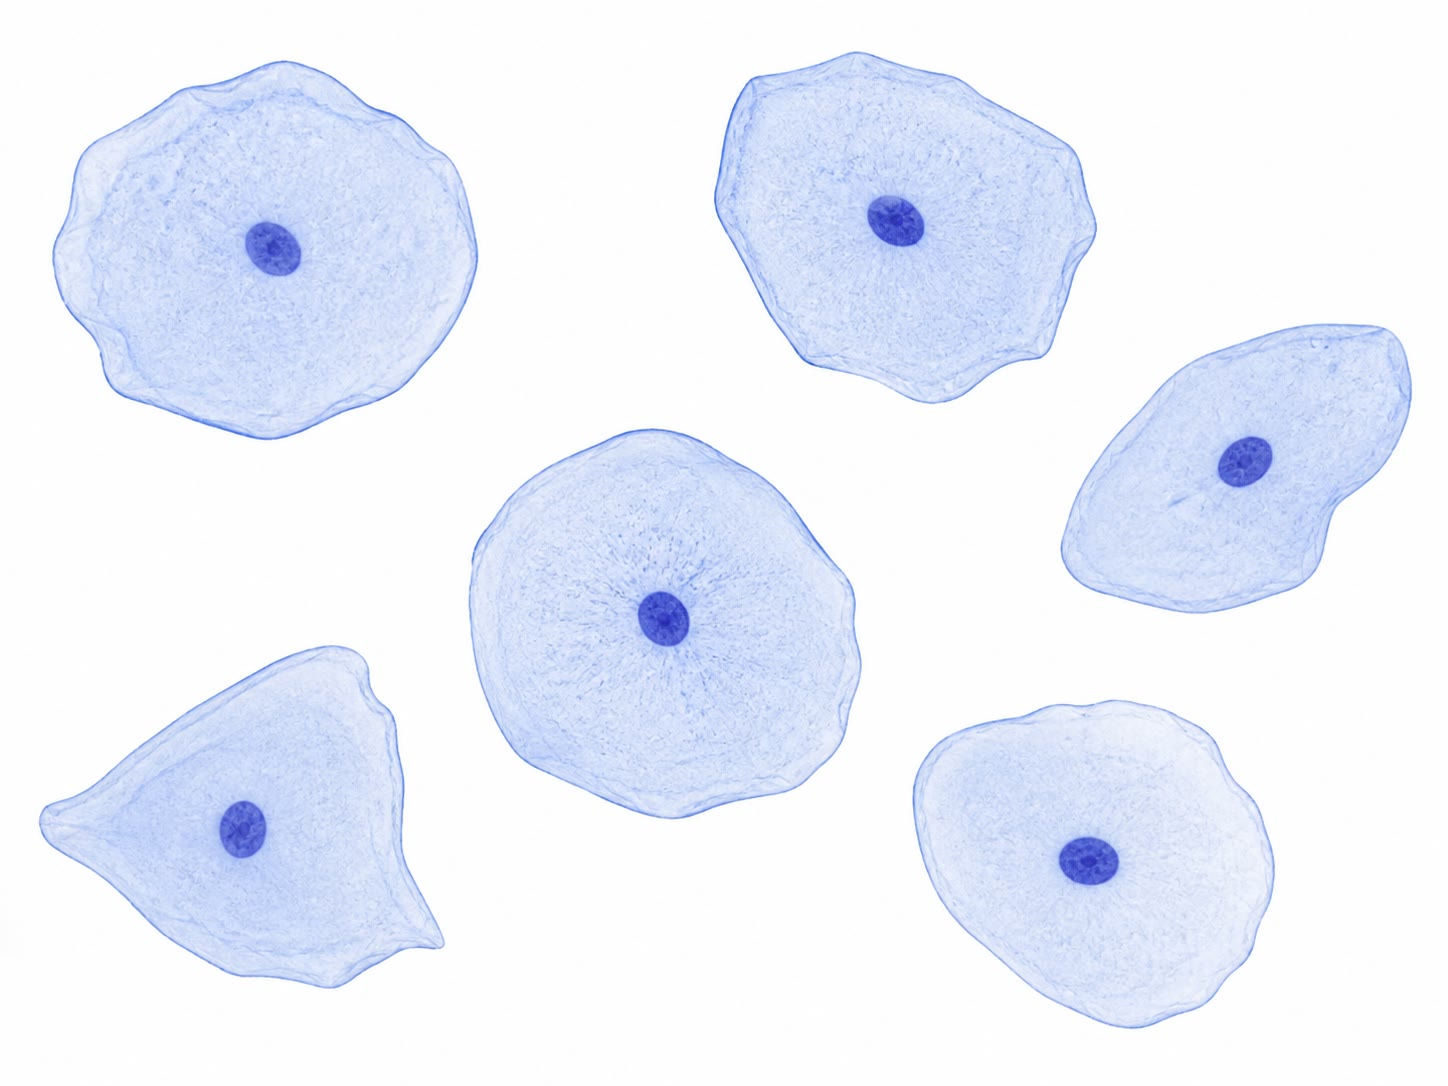
\includegraphics[width=\linewidth]{images/book1/ai/fig-cheek-cells.jpg}

{\small 口腔刮片：较圆的\omterm{def:g5:first-look-at-cells:cell}{细胞}，\\ 散开分布}
\end{minipage}

\medskip
{\small \omterm{def:g5:first-look-at-cells:microscope}{显微镜}下的洋葱\omterm{def:g5:first-look-at-cells:cell}{细胞}与口腔\omterm{def:g5:first-look-at-cells:cell}{细胞}。每个隔间——
连同其中的小暗点——都是一个\omterm{def:g5:first-look-at-cells:cell}{细胞}。}
\end{omfigure}

\begin{remark}[那个暗点]\label{rem:g5:first-look-at-cells:nucleus}
两幅图中，大多数\omterm{def:g5:first-look-at-cells:cell}{细胞}内部都有一个较暗的小点：
它是\omterm{def:g5:first-look-at-cells:cell}{细胞}的“指挥中心”，称为
\emph{细胞核}\index{细胞核}。\omterm{def:g5:first-look-at-cells:cell}{细胞}核所指挥的内容
——其中盘绕的那条著名的遗传指令链——是
本书后面几年的内容；现在只需注意，
这些小隔间并不是空的。
\end{remark}

\section{从一个细胞到一个身体}

\begin{proposition}[生物体靠细胞生长]\label{prop:g5:first-look-at-cells:growth}
\omterm{def:g1:living-or-not:living}{生物}体能够生长并自我修复，是因为它的\omterm{def:g5:first-look-at-cells:cell}{细胞}能够\emph{分裂}：
一个\omterm{def:g5:first-look-at-cells:cell}{细胞}分裂成两个活\omterm{def:g5:first-look-at-cells:cell}{细胞}，两个分裂成四个，依此类推。
长高
（见\cref{prop:g3:stages-of-life:animals}）本质上是\omterm{def:g5:first-look-at-cells:cell}{细胞}在增多；
伤口愈合
（见\cref{rem:g3:bones-and-muscles:alive}）则是\omterm{def:g5:first-look-at-cells:cell}{细胞}在重建。
而且，每一个身体，即使是最大的身体，都始于\emph{单个
\omterm{def:g5:first-look-at-cells:cell}{细胞}}——即
\cref{def:g4:animal-reproduction:sexual}中的\omterm{def:g4:animal-reproduction:sexual}{受精}\omterm{def:g4:animal-reproduction:sexual}{卵细胞}。
\end{proposition}
\admitted

\begin{example}[从一个到数万亿个]\label{ex:g5:first-look-at-cells:one}
\omterm{def:g4:animal-reproduction:sexual}{受精}卵分裂成 $2$ 个\omterm{def:g5:first-look-at-cells:cell}{细胞}，再变成 $4$ 个、$8$ 个，
$16$ 个 \dots{} 经过数月乃至数年的反复分裂，
才形成了此刻正在阅读这句话的你
身上的几十万亿个\omterm{def:g5:first-look-at-cells:cell}{细胞}。你身上的每一个\omterm{def:g5:first-look-at-cells:cell}{细胞}，都是从那第一个\omterm{def:g5:first-look-at-cells:cell}{细胞}繁衍而来的。
\end{example}

\begin{remark}[单细胞的完整生命]\label{rem:g5:first-look-at-cells:onecelled}
有些\omterm{def:g1:living-or-not:living}{生物}从不超过一个\omterm{def:g5:first-look-at-cells:cell}{细胞}——也
无需更多。一滴池塘水中挤满了它们：单个
\omterm{def:g5:first-look-at-cells:cell}{细胞}能游动、取食、分裂，正是显微尺度上的完整生命。
\cref{def:g1:healthy-habits:germs}中的\omterm{def:g1:healthy-habits:germs}{病菌}大多是
这类单\omterm{def:g5:first-look-at-cells:cell}{细胞}\omterm{def:g1:living-or-not:living}{生物}——老相识，
如今有了解释。
\end{remark}

\section{练习}

\begin{exercise}[$\star$]\label{exo:g5:first-look-at-cells:1}
什么是\omterm{def:g5:first-look-at-cells:cell}{细胞}？你的身体大约由多少个\omterm{def:g5:first-look-at-cells:cell}{细胞}组成？
\end{exercise}

\begin{exercise}[$\star$]\label{exo:g5:first-look-at-cells:2}
为什么在历史的大部分时间里，人们都不知道\omterm{def:g5:first-look-at-cells:cell}{细胞}？
是哪种仪器改变了这一点？
\end{exercise}

\begin{exercise}[$\star$]\label{exo:g5:first-look-at-cells:3}
描述\omterm{def:g5:first-look-at-cells:microscope}{显微镜}下洋葱表皮与口腔刮片所呈现的
情况，这两种观察结果有哪些共同之处？
\end{exercise}

\begin{exercise}[$\star$]\label{exo:g5:first-look-at-cells:4}
大多数\omterm{def:g5:first-look-at-cells:cell}{细胞}中可见的那个小暗点叫什么？
\end{exercise}

\begin{exercise}[$\star$]\label{exo:g5:first-look-at-cells:5}
大约多少个身体\omterm{def:g5:first-look-at-cells:cell}{细胞}排成一列，正好跨越一毫米——
一个\omterm{def:g5:first-look-at-cells:cell}{细胞}本身有多长，以毫米计？
\end{exercise}

\begin{exercise}[$\star$]\label{exo:g5:first-look-at-cells:6}
孩子长高时，\omterm{def:g5:first-look-at-cells:cell}{细胞}在体内做什么？
擦伤的膝盖愈合时呢？
\end{exercise}

\begin{exercise}[$\star$]\label{exo:g5:first-look-at-cells:7}
每个人的身体最初由多少个\omterm{def:g5:first-look-at-cells:cell}{细胞}开始？
由\cref{def:g4:animal-reproduction:sexual}可知，那第一个\omterm{def:g5:first-look-at-cells:cell}{细胞}是什么？
\end{exercise}

\begin{exercise}[$\star$]\label{exo:g5:first-look-at-cells:8}
一个\omterm{def:g5:first-look-at-cells:cell}{细胞}分裂为 $2$ 个，每一个又再次分裂，
依此类推。从 $1$ 个\omterm{def:g5:first-look-at-cells:cell}{细胞}开始继续倍增，经过
$5$ 次分裂后有多少个\omterm{def:g5:first-look-at-cells:cell}{细胞}？经过 $10$ 次呢？
\end{exercise}

\begin{exercise}[$\star\star$]\label{exo:g5:first-look-at-cells:9}
解释这句话：“雏菊与鲸鱼体现了
\omterm{prop:g5:first-look-at-cells:principle}{生命的统一性}。”根据
\cref{prop:g5:first-look-at-cells:principle}，它们有什么共同之处？
\end{exercise}

\begin{exercise}[$\star\star$]\label{exo:g5:first-look-at-cells:10}
一滴池塘水中含有若干\omterm{def:g1:living-or-not:living}{生物}，每个都只由
一个\omterm{def:g5:first-look-at-cells:cell}{细胞}构成。请对照\cref{prop:g1:living-or-not:signs}中的生命特征，
判断单个\omterm{def:g5:first-look-at-cells:cell}{细胞}
能表现哪些特征？
\end{exercise}

\begin{exercise}[$\star\star\star$]\label{exo:g5:first-look-at-cells:11}
大象的\omterm{def:g5:first-look-at-cells:cell}{细胞}与老鼠的\omterm{def:g5:first-look-at-cells:cell}{细胞}大小大致相同。
那么，使大象更大的是什么？是更大的\omterm{def:g5:first-look-at-cells:cell}{细胞}，还是
更多的\omterm{def:g5:first-look-at-cells:cell}{细胞}？根据\cref{prop:g5:first-look-at-cells:growth}，你的答案
说明了生长是如何进行的？
\end{exercise}
